\documentclass[11pt,letterpaper]{article}

% PAQUETES ++++++++++++++++++++++++++++++++
\usepackage[utf8]{inputenc}
\usepackage[spanish]{babel}
\usepackage{amsmath}
\usepackage{amsfonts}
\usepackage{amssymb}
\usepackage[left=2cm,right=2cm,top=2cm,bottom=2cm]{geometry}
\pagenumbering{arabic}
\usepackage[pdftex]{graphicx}
\usepackage{tabularx}
\usepackage{tcolorbox}
\usepackage{array}
\usepackage{url}
\usepackage{relsize}
\usepackage{multirow}
\usepackage{float}
\usepackage{tabularray}
\tcbuselibrary{most}
\decimalpoint

%+++++++++++++++++++++++++++++++++++++++++++++++++++
\graphicspath{ {./img/}}
\pagenumbering{arabic}
\newtcolorbox{matlab-code}[2][]{colback=red!3!white, colframe=red!75!black, colbacktitle=red!75!black, enhanced, attach boxed title to top center={yshift=-2mm}, title={#2}, #1}



% +++++++++++++++++++++
\begin{document}
\title{Trabajo de Investigación: Ajuste de Curvas por Mínimos Cuadrados}

\author{
	Alberto Ramos Cruz
	\and Moisés Alonso Marroquín Ayala
	\and René Eduardo Hernández Castro
	\and Roberto José Melgares Zelaya
}
\maketitle


\section{Regresión lineal por mínimos cuadrados}
%++++++++++++++++++
%PUNTO 1 A ALBERTO
%+++++++++++++++++++++++++
\subsection{Ajuste de una recta por regresión por mínimos cuadrados}
Esta es una técnica que, dados un conjunto de pares ordenados $(X,Y)$, nos permite adaptar una recta que se acerque lo más posible a todos los puntos de manera que represente de mejor forma una serie de datos. De esta forma minimizando la suma de los cuadrados de las diferencias entre los valores observados $Y$ y los valores predichos por la recta, reduciendo así la diferencia entre los datos reales y la recta adaptada, para esto se necesita utilizar la formula general de una recta: $$ y = mx + b$$
Donde se tiene que 
\begin{itemize}
	\item $y$ es el valor predicho por la formula como la variable dependiente.
	\item $x$ es el valor de la variable dependiente.
	\item $m$ es la pendiente de la recta.
	\item $b$ es la intersección de la recta con el eje $Y$.
\end{itemize}
Para método lo que se busca encontrar $m$ recurrimos a la fórmula:
\begin{equation}
m = \frac{\sum_{i=1}^{n} x_iy_i - \frac{\sum_{i=1}^{n} x_i \sum_{i=1}^{n} y_i}{n}}{\sum_{i=1}^{n} x_i^2 - \frac{(\sum_{i=1}^{n} x_i)^2}{n}}
\end{equation}
Por otro lado, para encontrar $b$ hacemos uso de la fórmula:
\begin{equation}
b = \frac{\sum_{i=1}^{n} y_i - m\sum_{i=1}^{n} x_i}{n}
\end{equation}
Donde $n$ representa la cantidad de datos que se tienen en la serie de pares ordenados. De esta manera se garantiza que la que se acerca lo mas posible a todos los puntos, minimizando el error cuadrático, y reflejando de manera más precisa la relación entre las variables.\cite{nieves2011metodos} \par A continuación, se demuestra un ejercicio resuelto haciendo uso del método anterior junto con un algoritmo en \textit{MATLAB}
\subsubsection{Ejercicio propuesto haciendo uso del método de ajuste de recta por mínimos cuadrados}
\begin{center}
\textit{\textbf{Ejercicio 1: } En la siguiente tabla, T es la temperatura de una bobina en °C  y r es la resistencia de la bobina en Ohms ($\Omega$). Ajuste una recta de mínimos cuadrados para representar r en términos de T. Estime cual sería la resistencia de una bobina que está a 65 °C. Posteriormente, grafique la recta de mínimos cuadrados y los puntos de la tabla en un solo plano cartesiano}.\linebreak \par
\begin{tabular}{c|cccccc}
 \hline 
 T (°C) & 10.50 & 29.49 & 42..70 & 60.01 & 75.51 & 91.05 \\ 
 \hline 
 r ($\Omega$) & 10.421 & 10.939 & 11.321 & 11.794 & 12.242 & 12.668 \\ 
 \hline 
 \end{tabular} 
\end{center}
Para este problema nuestra \textit{variable independiente} serán los valores de la temperatura \textit{T}, mientras que nuestra \textit{variable dependiente} serán los valores de la resistencia, por ello los valores de $X$ y $Y$ serán la temperatura y la resistencia, respectivamente. Comenzamos el algoritmo en \textit{MATLAB} agregando los datos iniciales y realizando las primeras sumas de los valores de $X$, $Y$,  $X^2$, y $XY$, sabiendo que $n = 6$. 

\begin{figure}[H]
\begin{tcolorbox}[title = Problema 1: Declaración de valores iniciales y sumatorias]
\begin{verbatim}
T = [10.50 29.49 42.70 60.01 75.51 91.05]; % X - variable independiente
R = [10.421 10.939 11.321 11.794 12.242 12.668]; % Y variable dependiente
n = length(T);

sumatoriaX = sum(T); % sumatoria de X
sumatoriaY = sum(R); % sumatoria de Y
multiXY=0; % Para la sumatoria de XY
X2=0; % Para la sumatoria de X^2

for i=1:n
    multiXY = multiXY+(T(i)*R(i));
    X2 = X2 + T(i)^2;
end
\end{verbatim}
\end{tcolorbox}
\end{figure}
Con los valores encontrados de las sumas, podemos pasara  encontrar $m$ y $b$ para luego armar la función lineal de $r=mt + b$
\begin{figure}[H]
\begin{tcolorbox}[title = Problema 1: Armando la función lineal de aproximación]
\begin{verbatim}
% Obteniendo la pendiente en mi función y=mx+b que se reescribe como r = mT+b
m = (multiXY-((sumatoriaX*sumatoriaY)/n))/(X2-(sumatoriaX^2/n));

% Obteniendo el intersecto b de la función
b = (sumatoriaY-(m*sumatoriaX))/n;

%se escribe la función
syms t;
r = m*t+b;
\end{verbatim}
\end{tcolorbox}
\end{figure}

Con las líneas anteriores se obtienen finalmente los valores de la pendiente y el intercepto de la función lineal que se puede usar para aproximar valores. 
\begin{figure}[H]
\centering
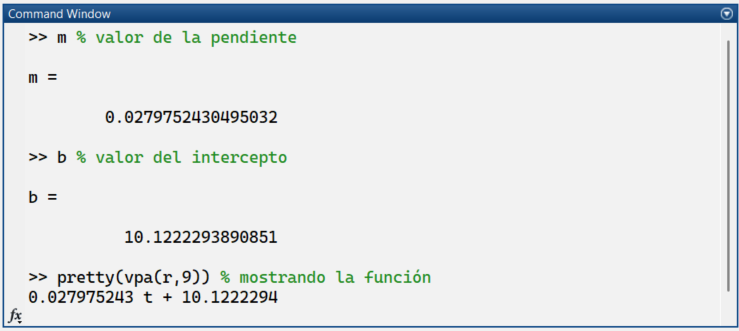
\includegraphics[width=4.5in]{eq1.png}
\caption{Los valores de $b$ y $m$ obtenidos con el algoritmo junto con la función}
\label{figure:lineal1} 
\end{figure}
Ahora es posible obtener la estimación deseada de la resistencia a una temperatura de 65 °C haciendo uso del comando \texttt{double(subs(r,65))}. Para finalizar el ejercicio, mostraremos como la gráfica de la recta se sobrepone a los valores iniciales provistos por el ejercicio. 
% resultado
\begin{figure}[H]
\centering
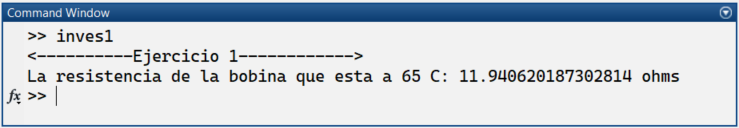
\includegraphics[width=4in]{res1.png}
\caption{Resultado de la evaluación de la función $r=mt + b$ en 65, obteniendo así una respuesta de \textbf{11.940620187302814 ohms}}
\label{figure:res1}
\end{figure}
%grafica
\begin{figure}[H]
\centering
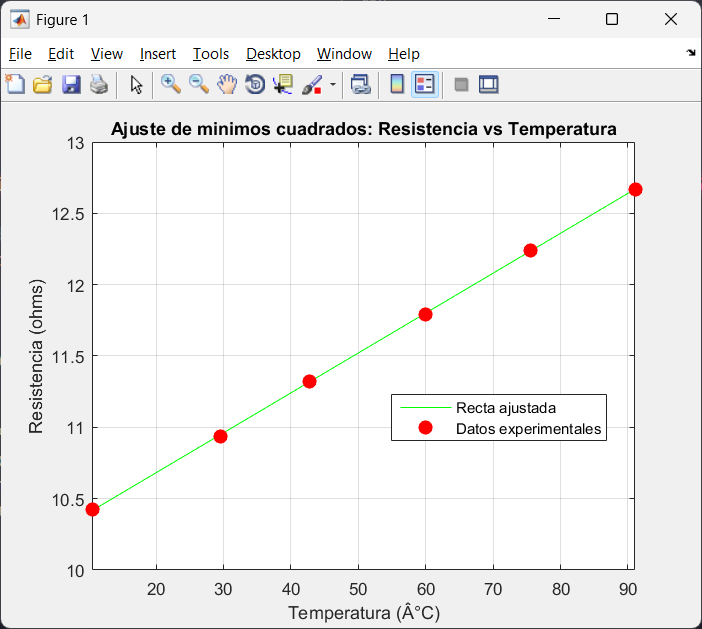
\includegraphics[width=3.5in]{recta.png}
\caption{Gráfica de la recta obtenida con el método de estudio con los valores iniciales de la temperatura y la resistencia sobre la misma. }
\label{figure:recta1}
\end{figure}

%---------------
%PUNTO 1 B // RENE
%---------------
\subsection{Linealización de relaciones no lineales}
Una función $y$ se puede formar mediante la combinación de múltiples funciones lineales $f_1$,$f_1$,\dots,$f_n$y la minimización de la suma de los cuadrados de las diferencias entre la predicción del modelo y los datos generados en un sistema lineal de ecuaciones para los coeficientes del modelo. Si se construye de esta forma "y" es lineal en sus coeficientes. En este caso analizaremos la posibilidad de convertir relaciones no lineales a su forma lineal de forma similar al método descrito anteriormente.\cite{ualberta} Consideraremos los siguientes modelos:
\begin{itemize}
	\item Modelo Exponencial $y = \alpha e^{\beta x}$
	\item Modelo Exponencial $y = \alpha x^{\beta}$
\end{itemize}
\par Este tipo de modelos no lineales en $x$ y sus coeficientes desconocidos $\beta$ y $\alpha$ se pueden transformar en modelos no lineales mediante el uso de logaritmo natural. Aplicando logaritmo natural a los modelos nos queda:
\begin{itemize}
	\item Modelo Exponencial ($y = \alpha e^{\beta x}$) $\longrightarrow$ $\beta x + \ln \alpha$
	\item Modelo Exponencial ($y = \alpha x^{\beta}$) $\longrightarrow$ $\beta \ln x + \ln \alpha$
\end{itemize}
\par 
En el caso del modelo exponencial se puede convertir como $(x_i, \ln(y_i))$ y con ello se puede hacer uso de la regresión lineal  para encontrar los coeficiente $\beta$ y $\alpha$. Para el caso del modelo potencial la información se puede expresar como $(\ln(x_i), \ln(y_i))$ y nuevamente hacer uno de la regresión lineal para encontrar los coeficientes $\beta$ y $\alpha$.\cite{ualberta}\cite{nieves2011metodos} 

\subsubsection{Coeficiente de determinación para relaciones no lineales}
Para determinar que tan los datos se ajustan al modelo se hará uso del ``coeficiente de determinación'' , si bien este coeficiente puede variar dependiente que software o articulo se esta obteniendo, en nuestro caso haremos uso de lo siguiente:
\begin{equation}\label{equation:coeficiente}
	R^2 = 1 - \frac{\sum_{i=1}^{n} (y_i - y(x_i ) ^2 }
	{\sum_{i=1}^{n} (y_i)^2}
\end{equation}

Donde $R^2$ es equivalente a 1 menos el coeficiente entre la suma de cuadrados del modelo y la suma total de cuadrados de los datos. Esta definición de $R^2$ es la mas común usada para modelos no lineales. Para describir dicha definición y lo descrito anteriormente para convertir ambos modelos exponencial y potencial en relaciones líneas se hará los siguientes ejemplos:

\subsubsection{Método Exponencial}
Recordando la forma exponencial, $y = \alpha e^{\beta x}$, es posible linealizarla mediante el uso de logaritmo natural para obtener la forma $\beta x + \ln \alpha$ y convertir una serie de datos a $(x_i, \ln(y_i))$. En el caso del modelo potencial, recordando su forma $y = \alpha e^{\beta x}$, se debe de linealizar también haciendo uso de logaritmo natural obteniendo $\beta \ln x + \ln \alpha$ , con ello convertiremos los datos a la forma final $(\ln(x_i), \ln(y_i))$.  \cite{ualberta}
\par
Mediante el uso de regresión lineal es posible expresar $y*$ como: \textbf{$y* = \beta^* x + \alpha^*$ 	} obtendremos los coeficientes $\alpha^*$ y $\beta^*$ de la siguiente manera:
\begin{align*}
	\beta^* &= \frac{n \sum_{i=1}^{n} x_iy_i^* - \sum_{i=1}^{n} x_i \sum_{i=1}^{n} y_i^*}{n\sum_{i=1}^{n} x_i^2 - (\sum_{i=1}^{n}  x_i)^2} \\
	\alpha^* &= \frac{\sum_{i=1}^{n} y_i^* - b^* \sum_{i=1}^{n} x_i  }{n} \\
\end{align*}
Para el modelo potencial, es necesario sustituir los valores $x_i$ en la formula por las $x^*$ que corresponden a la evaluación de $\ln(x_i)$.
Con el uso de \textit{MATLAB} u otro método analítico, obtenemos los datos para utilizar en los cálculos de las ecuaciones anteriores.s
% AAAAAAAAAAAAAAAAAAAAAAAA METODO POTENCIAL
\subsection{Método Potencial}


%---------------
%PUNTO 2
%---------------
\section{Aproximación polinomial con mínimos cuadrados}
Con el fin de encontrar un modelo matemático que represente lo mejor posible a una serie de datos experimentales, es posible abordarlo por medio de una curva $y=\phi(x)$ que se aproxime a los datos, sin la necesidad de que esta curva pase por ellos.
Lo anterior plantea el problema de verificar que en los términos:
$\{(x_i, y_i)\quad i = 0,1,2,3, \cdots, N\} $ se debe de hallar un $\phi(x)$ que verifique

$$Minima = \sum_{i=0}^{N} (y_i - \phi(x_i))^2$$

Para evitar problemas se suele utilizar una diferencia cuadrada para evitar problemas de derivabilidad. 
\subsection{Parábola de mínimos cuadrados}
La parábola de mínimos cuadrados tiene como objetivo aproximar un conjunto de puntos 
$(x_0, y_0),$ $(x_1, y_1),$ $ (x_2, y_2),$ $ \cdots , (x_n, y_N)$, donde $N$ es el número de elementos en el conjunto de puntos, 
a través de una curva polinomial de grado 2. Entonces, podemos entender la parábola de mínimos cuadrados como una curva de $y=\phi(x)$ donde $\phi(x)$ es un polinomio de segundo grado que viene dado por la ecuación
$$y = a_0 + a_1 x + a_2 x^2  $$
donde $a_0, a_1, a_2 \in R$ y se determinan resolviendo las ecuaciones simultaneas : 

\begin{equation} \label{eq:sist-parab} 
	\left\{
		\begin{array}{@{}l@{}}
			\sum_{i=0}^{N} y_i  = a_0N + a_1\sum_{i=0}^{N} x_i + a_2\sum_{i=0}^{N} x_i^2 \cr\cr
			\sum_{i=0}^{N} x_iy = a_0\sum_{i=0}^{N} x_i + a_1\sum_{i=0}^{N} x_i^2 + a_2\sum_{i=0}^{N} x_i^3 \cr\cr
			\sum_{i=0}^{N} x_i^2y = a_0\sum_{i=0}^{N} x_i^2 + a_1\sum_{i=0}^{N} x_i^3 + a_2\sum_{i=0}^{N} x_i^4 		
		\end{array}
	\right.
\end{equation}
\linebreak 
Las ecuaciones anteriores  son conocidads como \textit{ecuaciones normales de mínimos cuadrados}. Estas ecuaciones se obtienen al multiplicar la ecuación $y = a_0 + a_1 x + a_2 x^2  $ por  1, $x$, y $x^2$, respectivamente. Como se puede observar, se obtiene un \emph{sistema con 3 incógnitas y 3 ecuaciones.}
\par
Para obtener los valores que acompañan a las incógnitas $a_i$ en el sistema de ecuaciones se debe de obtener la suma de los productos, tomando en cuenta los valores respectivos de $x_i$ con sus imágenes en $y_i$; esto a excepción del valor $N$ que acompaña a la incógnita $a_0$ en la primera ecuación como se puede observar en la Ecuación \ref{eq:sist-parab}.
\par
A continuación, se procede a resolver el sistema de ecuaciones por medio de una matriz de 4$\times$3 para que de esste modo se obtengan los valores de las 3 incógnitas. \cite{spiegel}\cite{nieves2011metodos} En este caso, se puede usar cualquier método de resolución de sistemas de ecuaciones por medio de matrices, aunque para esta investigación se hará uso del método de Cramer. \emph{ Con el objetivo de mejorar la comprensión lectora, a partir de este punto se usará la siguiente notación.}

 \begin{table}[H]
 \centering
	\begin{tabular}{ c | c }
	\hline
	Símbolo & Significado  \\ \hline
	$X$ &	$\mathlarger{\Sigma} x_i$  \\ 
	$Y$ &   $\mathlarger{\Sigma} y_i$ \\
	$X^2$ & $\mathlarger{\Sigma} x_i^2$ \\
	$X^3$ & $\mathlarger{\Sigma }x_i^3$ \\ 
	$X^4$ & $\mathlarger{\Sigma} x_i^4$ \\
	$XY$ &  $\mathlarger{\Sigma} x_i y_i$	\\
	$X^2Y$& $\mathlarger{\Sigma} x^2_i y_i$	\\ \hline
	\end{tabular}
	\label{table:simbologia}
\end{table}

Usando la notación anterior, pasamos a resolver la matriz y obtener las ecuaciones que nos dan los determinantes. \emph{Recordar que estas matrices no contienen variables simbólicas, sino que valores escalares representados con letras mayúsculas.}
\begin{table}[H] \centering \begin{tabular}{c c c c c}
%% resolucion a0
$a_0 = \frac{
		\begin{vmatrix}
		 	Y &	X	& X^2 \\
		 	XY &	X^2	& X^3 \\
		 	X^2Y & X^3 & X^4	 
		\end{vmatrix}}
		{\begin{vmatrix}
		 	N &	X	& X^2 \\
		 	X &	X^2	& X^3 \\
		 	X^2 & X^3 & X^4	 
		\end{vmatrix}}
		
$ & &
% resolucion a1
$ a_1 = \frac{
		\begin{vmatrix}
		 	N &	Y	& X^2 \\
		 	X &	XY	& X^3 \\
		 	X^2 & X^2Y & X^4 
		\end{vmatrix}}
		{\begin{vmatrix}
		 	N &	X	& X^2 \\
		 	X &	X^2	& X^3 \\
		 	X^2 & X^3 & X^4	 
		\end{vmatrix}}
$ & &
% resolucion a2
$ a_2 = \frac{
		\begin{vmatrix}
		 	N &	X	& Y \\
		 	X &	X^2	& XY \\
		 	X^2 & X^3 & X^2Y 
		\end{vmatrix}}
		{\begin{vmatrix}
		 	N &	X	& X^2 \\
		 	X &	X^2	& X^3 \\
		 	X^2 & X^3 & X^4	 
		\end{vmatrix}}
$ \\
\end{tabular} \end{table}
%% PROBLEMA 4
\subsubsection{Ejercicio propuesto usando el método de la parábola de mínimos cuadrados}
A continuación se presenta el siguiente problema:
\begin{center}
	\textit{\textbf{Problema 4:} En la investigación de accidentes automovilísticos, el tiempo total requerido para el frenado total de un automóvil después de que el conductor ha percibido un peligro está compuesto de su tiempo de reacción (el tiempo que transcurre en su detección del peligro y la aplicación de los frenos) más el tiempo de frenado (el tiempo que tarda el automóvil en detenerse después de la aplicación de los frenos). La siguiente tabla proporciona la distancia de frenado D en metros de un automóvil que viaja a diversas velocidades V en metros por segundo al momento en el cual el conductor detecta un peligro.}
	\linebreak\par
	\begin{tabular}{c| c c c c c c }
	\hline
		Velociad V(m/s) &   20 & 30 & 40 & 50 & 60 & 70 \\ 		\hline
		Distancia de frenado D(m) & 54 & 90 & 138 & 206 & 292 & 396 \\
		\hline
	\end{tabular}
	\begin{itemize}
		\item \textbf{a)} Encontrar la ecuación de la parábola de mínimos cuadrados que ajuste esta serie de datos.
		\item \textbf{b)} Estimar la distancia $D$ de frenado cuando el automóvil se esta desplazando a 55 m/s y a 75 m/s.
		\item \textbf{c)} Grafique la paráboa y los puntos de la tabla en un mismo plano cartesiano.
	\end{itemize}
\end{center}

Para resolver este problema haremos uso de \emph{MATLAB} de la siguiente forma. En este caso las $X$ las usaremos como los valores $V$ de velocidad, mientras que los valores de $Y$ serán la distancia $D$
%Implementacion matlab1
\begin{figure}[H]
\begin{tcolorbox}[title=Problema 4: Implementación en MATLAB]
	\begin{verbatim}
		%% Declarando los arreglos de los valores
		X = [20, 30, 40, 50, 60, 70]
		Y = [54, 90, 138, 206, 292, 396]
		suma_X = 0; suma_X2 = 0;
		suma_X3 = 0; suma_X4 = 0;
		suma_Y = 0; suma_XY = 0;
		suma_X2Y = 0;
		N = length(X); % Tamaño de la matriz de X
		% Sumas de cada uno de los valores que se usaran para armar la matriz 
for i = 1: N
    suma_X = suma_X + X(i); % Suma Xi
    suma_X2 = suma_X2 + X(i) ^ 2; % Suma Xi^2
    suma_X3 = suma_X3 + X(i) ^ 3; % Suma Xi^3
    suma_X4 = suma_X4 + X(i) ^ 4; % Suma Xi^4
    suma_Y = suma_Y + Y(i); % Suma Yi
    suma_XY = suma_XY + X(i) * Y(i); % Suma Xi * Yi
    suma_X2Y = suma_X2Y + X(i) ^ 2 * Y(i); % Suma Xi^2 * Yi
end
\end{verbatim}
\end{tcolorbox}
\end{figure}
Con esto podemos armar la matriz  \texttt{M} , y la submatriz \texttt{subM}, que contendrán la matriz principal con los datos de las sumas de X, y los valores de los resultados respectivamente. A su vez, haremos uso de una matriz auxiliar \texttt{Maux} que será una copia de la matriz original, con los valores de la submatriz \texttt{subM} en una de las columnas como lo requiere el método de determinantes.
%matlab3
\begin{figure}[H]
\begin{tcolorbox}[ title=Problema 4: Implementación en MATLAB]
		\begin{verbatim}
		%% Creacion de la matriz M y submatriz subM
M = [ N suma_X suma_X2; suma_X suma_X2 suma_X3; suma_X2 suma_X3 suma_X4];
subM = [suma_Y suma_XY suma_X2Y];

%% encontrando los valores de a0, a1 y a2.
for i = 1:3
    Maux = M; %matriz auxiliar copia la original
    Maux(:,i) = subM; % reemplaza los valores de la columna
    a(i) = det(Maux) / det(M); % denominador del auxiliar con el de la original
end
		\end{verbatim}
		\end{tcolorbox}
		\centering
		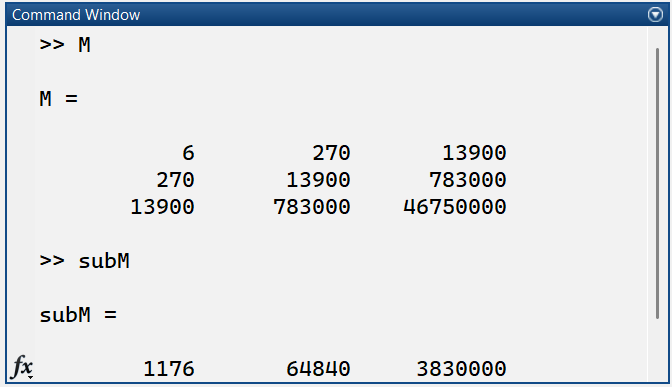
\includegraphics[width=2.8in]{mtz4.png}

\end{figure}
La demostración anterior queda resuelta la matriz y obtenemos los valores de $a_n$ (es de notar al lector que \textit{MATLAB} cuenta los arreglos y matrices desde el 1 por lo que \texttt{a(1)	} es igual a $a_0$) los cuales son: \par. 
\begin{align*}
a_0 &= 41.771428571430754 \\
a_1 &= -1.095714285714397 \\
a_2 &= 0.087857142857144 \\
\end{align*}
Con la matriz resuelta, junto con el arreglo con los valores de $a_0$, $a_1$ y $a_2$ podemos armar el polinomio en \textit{MATLAB} para resolver los incisos \textbf{a)} y \textbf{b)} evaluando la ecuación en los valores asignados. Por lo cual la ecuación de parábola que aproxima los datos es: 
$$P^2(x) =  41.771428571430754  - 1.095714285714397x + 0.087857142857144x^2$$ 

\begin{figure}[H]
\begin{tcolorbox}[title=Problema 4: Implementación en MATLAB]
\begin{verbatim}
syms x;
P = a(1) + a(2) * x  + a(3) * x ^ 2;
aprox = subs(P, v); % v es el valor de la velocidad al que deseamos aproximar
\end{verbatim}
\end{tcolorbox}
\end{figure}
Ahora que tenemos evaluado el polinomio que describe la parábola, podemos evaluarlo en los valores para $x=55$ y $x=75$ para obtener una aproximación de la distancia requerida a esas velocidades, propuestas por el literal \textbf{b)}. Por lo tanto obtenemos las siguientes evaluaciones en el polinomio \texttt{P} en \textit{MATLAB}:
\begin{figure}[H]
\centering
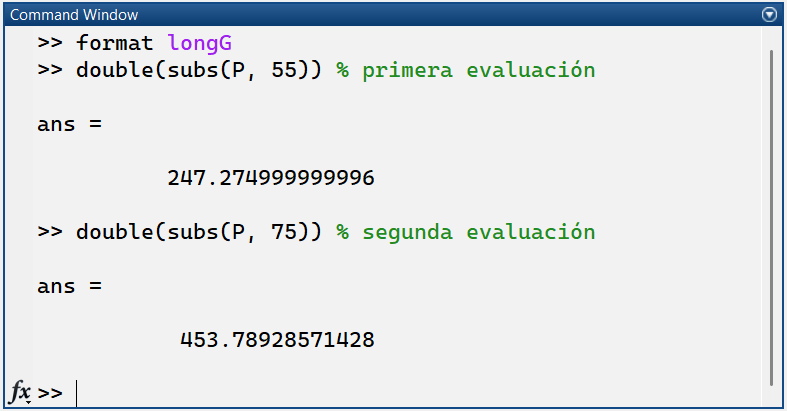
\includegraphics[width=3.5in]{res4.png}
\end{figure}
A continuación se muestra como los valores iniciales como se indica en el literal \textbf{c)} se ven sobre la parábola creada. Donde se muestran los valores iniciales sobre la parábola construida:
\begin{figure}[H]
\centering
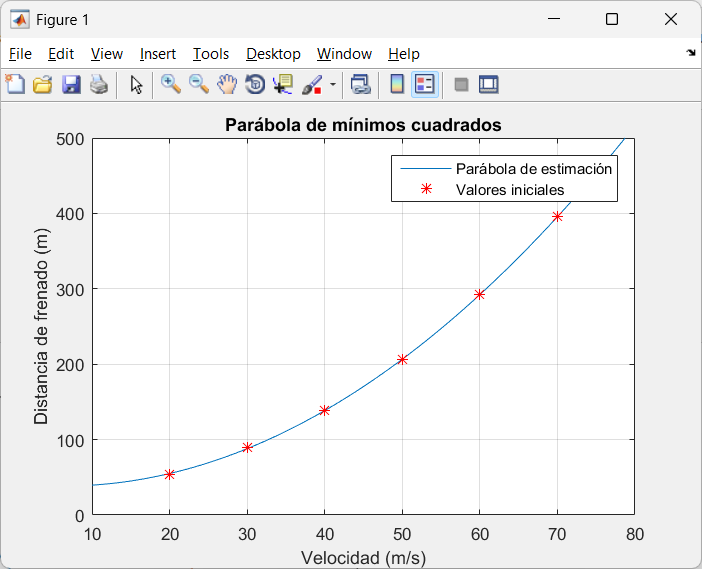
\includegraphics[width=4in]{parab4.png}
\end{figure}

% ++++++++++++++++++++++++
% SECCION 2B
%++++++++++++++++++++++++
\subsection{Ajuste de polinomios de grado \textit{n}	 (caso general)}
Si se desea aproximar una función dada de la forma tabular (pares x, y), de un polinomio grado N se realiza un procedimiento bastante similar al caso de la parábola de mínimos cuadrados. Para esto se debe minimizar la siguiente función:
\begin{equation} \label{	equation:ajustte}
	\sum_{i=1}^{m} \quad [ a_0 + a_1x_i + a_2x_i^2 + \dots + a_nx_i^n - f(x_i)] ^ 2
\end{equation}
\par
Para minimizar la función se debe derivar parcialmente con respecto a cada coeficiente $a_i$ desde 0 hasta $n$, para luego igualar a cero cada una de las funciones que se obtengan. De esta forma se llegará al siguiente sistema de ecuaciones lineales.
\begin{align*}
	ma_0 + a_1\Sigma x + a_2\Sigma x^2 + \dots + a_n\Sigma x^n &= \Sigma y \\
	a_0\Sigma x + a_1\Sigma x^2 + a_2\Sigma x^3 + \dots + a_n\Sigma x^{n+1} &= \Sigma xy\\
	a_0\Sigma x ^2 + a_1\Sigma x^3 + a_2\Sigma x^4 + \dots + a_n\Sigma x^{n+2} &= \Sigma x^2y \\
	\dots  & \dots \\
	a_0\Sigma x^n + a_1\Sigma x^{n+1} + a_2\Sigma x^{n+2} + \dots + a_n\Sigma x^{2n} &= \Sigma  x^ny
\end{align*}
\par
Una vez obtenido este sistema de ecuaciones se puede resolver mediante matrices o cualquier otro método de resolución de sistemas de ecuaciones.
\par  Una vez encontrados los valores de todos los coeficientes se puede crear el polinomio de la forma  $p(n) = a_0 + a_1x + a_2x^2 + a_3x^3 + \dots + a_nx^n$ . Este es una expansión del método anterior que se desarrolló, puesto que a partir de esta forma general se puede obtener el caso de la parábola cuando se trabaja con un polinomio de grado $n = 2$.\cite{nieves2011metodos} A continuación, se muestra un ejemplo práctico para su comprensión junto con un algoritmo de resolución en \textit{MATLAB}.
\begin{center}
\textit{\textbf{Ejemplo 2:} El calor específico $C_p$ (cal/kg mol) del $Mn_3O_4$ varía con la temperatura. A partir de la siguiente tabla, aproxime la información con un polinomio por el método de mínimos cuadrados.} \cite{nieves2011metodos}
\linebreak \par
	\begin{tabular}{c|c c c c c c}
	\hline 
	T (°K) & 280 & 650 & 1000 & 1200 & 1500 & 1700 \\ \hline
	$C_p$ (cal/kg mol) & 32.7 & 45.4 & 52.15 & 53.7 & 52.9 & 50.3 \\ 
	\hline 
	\end{tabular} 
\end{center}

Se hará uso del siguiente algoritmo en \textit{MATLAB} para mostrar el resultado de este método con $n=4$
\begin{figure}[H]
\begin{tcolorbox}[title=Ejemplo 2: Implementación en MATLAB]
\begin{verbatim}
syms x;
X = [280 650 1000 1200 1500 1700];
Y = [32.7 45.4 52.15 53.7 52.9 50.3];
xEvaluar = 1500;
%n se ocupará para indicar el grado del polinomio
n = 4;
% Guardar el valor de la sumatoria de Y
sumY = 0;
for j=1:length(Y)
   sumY = sumY + Y(j); 
end
%Guardar en un vector las sumas de todos los valores de X elevadas a sus
%potencias desde 1 hasta 2n 
for i=1:2*n
    sum = 0;
   for j=1:length(X)
       sum = sum + (X(j))^i;
   end
   sumXs(i) = sum;
end
%Creando un vector que almacene los resultados de la matriz
for i=1: n+1
    if i == 1
        resM(i) = sumY; 
    else
        sumatoria = 0;
        for j=1:length(X)
             sumatoria = sumatoria + Y(j)*X(j)^(i-1);
        end
        resM(i) = sumatoria;
    end
end
\end{verbatim}
\end{tcolorbox}
\end{figure}
El algoritmo anterior nos ayuda a dar las sumas de los valores requeridos, los cuales son almacenados dentro de una matriz \texttt{sisM} como veremos a continuación donde se llenaran todas sus filas. La matriz resultante en \textit{MATLAB }se muestra en la \textit{Figura \ref{figure:sisM}}.

\begin{figure}[H]
\begin{tcolorbox}[title=Ejemplo 2: Implementación en MATLAB]
\begin{verbatim}
k = length(resM);
sisM = zeros(k);
for j=1:k %Llenando la primera fila
    if j == 1
        sisM(j,j) = length(X);
    else
        sisM(1,j) = sumXs(j-1);
    end
end
for i=2:k % Llenando el resto de filas
   for j=1:k
       if(i == 2)
           sisM(i,j) = sumXs(j);
       else
           sisM(i,j) = sumXs(i+j-2);
       end
   end
end
sisM(k,k) = sumXs(2*n);
\end{verbatim}
\end{tcolorbox}
\end{figure}
\begin{figure}[H]
\centering
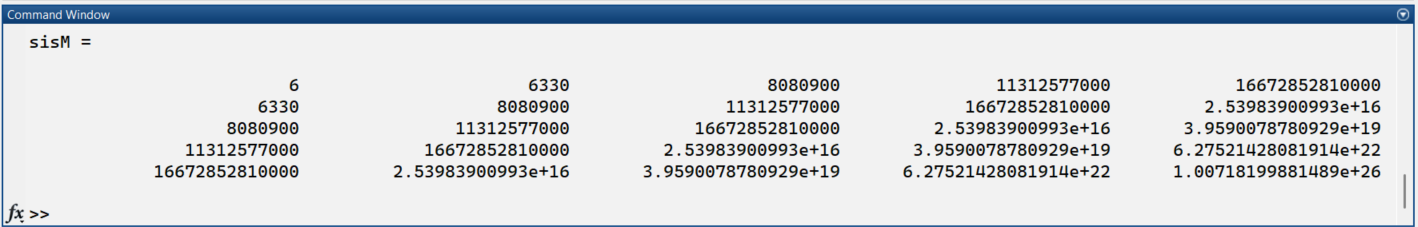
\includegraphics[width=6in]{sisM.png}
\label{figure:sisM}
\end{figure}
Con la matriz creado es momento de pasar a resolver el sistema para obtener los coeficientes del polinomio y posteriormente, la respuesta al problema.
\begin{figure}[H]
\begin{tcolorbox}[title=Ejemplo 2: Implementación en MATLAB]
\begin{verbatim}
%Resolver el sistema de ecuaciones
detM=det(sisM); % lo guardamos para no requerir calcularlo siempre
for i=1:k
   newMatrix = sisM;
   newMatrix(:,i) = resM;
   coeficientes(i) = det(newMatrix)/detM;
end
% Generando el polinomio
pol = coeficientes(1);
for i=2:k
    pol = pol + coeficientes(i)*x^(i-1);
end
estimacion = double(subs(pol,xEvaluar)); %% Respuesta
\end{verbatim}
\end{tcolorbox}
\end{figure}
\begin{figure}[H]
\centering
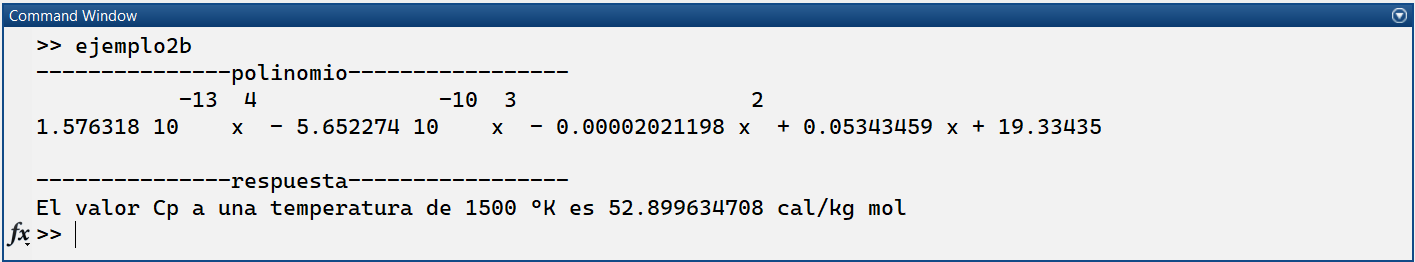
\includegraphics[width=6in]{ej2ans.png}
\label{figure:ans2}
\end{figure}



%+++++++++++++++++++++++
% BIBLIOGRAFIA
% +++++++++++++++++++++++
\bibliographystyle{IEEEtran}
\bibliography{bibi}
\end{document}